\documentclass{article}
\usepackage[utf8]{inputenc}
\usepackage[T1]{fontenc}
\usepackage[brazil]{babel}
\usepackage{geometry}
\usepackage{amsmath}
\usepackage{ragged2e}
\usepackage{listings}
\usepackage{graphicx}
\graphicspath{ {graficos/} } % <-- Posição correta e recomendada
\usepackage{float}
\usepackage{xcolor}
\usepackage{booktabs}
\usepackage{multirow}

% Hyperref deve ser um dos últimos pacotes carregados
\usepackage[colorlinks=true, 
            linkcolor=blue, 
            urlcolor=blue, 
            citecolor=blue]{hyperref}

\geometry{a4paper, left=3cm, right=2cm, top=3cm, bottom=2cm}
\setlength{\parindent}{1.25cm}

\lstset{
    language=Python,                % Define a linguagem para syntax highlighting
    basicstyle=\ttfamily\small,     % Usa fonte monoespaçada e um pouco menor
    keywordstyle=\color{blue},          % Cor para palavras-chave
    commentstyle=\color{gray},      % Cor para comentários
    stringstyle=\color{orange},         % Cor para strings
    showstringspaces=false,         % Não mostra espaços em strings com um símbolo especial
    breaklines=true,                % <<< ESSA É A OPÇÃO PRINCIPAL: Quebra as linhas automaticamente
    breakatwhitespace=true,         % Tenta quebrar as linhas nos espaços em branco
    frame=single,                   % Desenha uma caixa simples ao redor do código
    rulecolor=\color{black!30},     % Cor da caixa
    numbers=left,                   % Coloca números de linha à esquerda
    numberstyle=\tiny\color{gray},  % Estilo dos números de linha
    captionpos=b,                   % Posição da legenda (b=bottom)
    tabsize=4,                      % Tamanho da tabulação
    postbreak=\mbox{\textcolor{red}{$\hookrightarrow$}\space} % Símbolo para indicar quebra de linha
}
\begin{document}

\begin{titlepage}
    \centering
    
\includegraphics[width=0.4\textwidth]{brasao_ufba.jpg} \\
    \vspace{1cm}
    
    \textbf{\large UNIVERSIDADE FEDERAL DA BAHIA} \\
    \vspace{12cm}
    
    \textbf{\large Salvador - BA} \\
    \textbf{\large 2025}
\end{titlepage}




\begin{center}
\large\textbf{Avaliação 2 - Métodos Numéricos - 2025.1} \\
\end{center}

\begin{flushleft}
Aluno: Guilherme Rocha Ribeiro \\
Professor: Reiner Requião \\
Matéria: ENGG03
\end{flushleft}

\section*{Questão 1: Modelagem de dois tanques acoplados}
\justifying
\begin{equation}\label{eq:sistema}
\begin{cases}
\frac{dh_1}{dt} = -a\sqrt{h_1} + b(h_2 - h_1) \\
\frac{dh_2}{dt} = a\sqrt{h_1} - b(h_2 - h_1) \\
\end{cases}
\end{equation}
Baseado nessa modelagem foi possível identificar que esse sistema, ao decorrer do tempo, chega a um estado estacionário.
\subsection*{Resultados}
\begin{figure}[H]
        \centering
        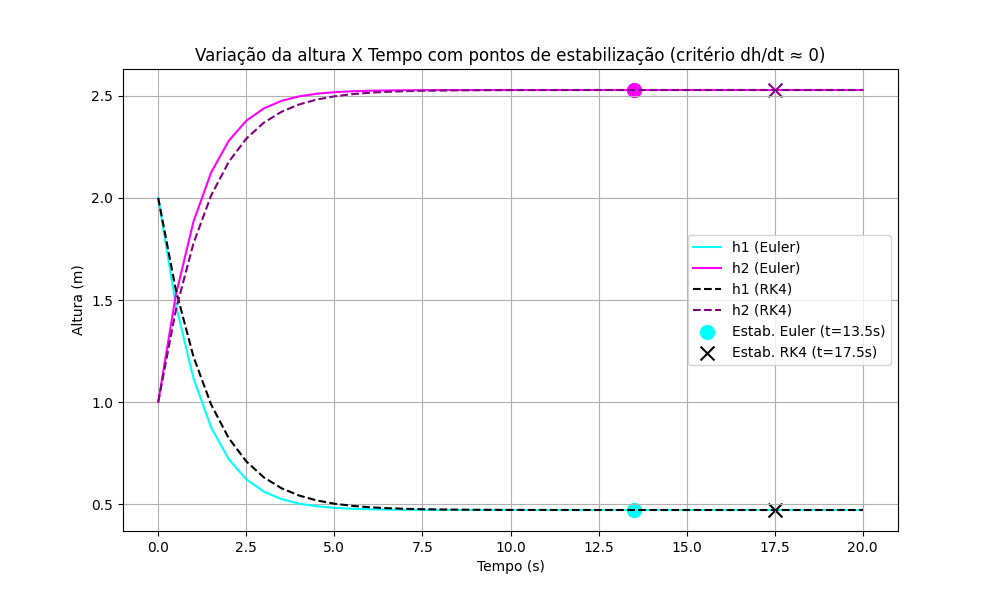
\includegraphics[width=1\textwidth, height=0.3\textheight, keepaspectratio]{Q1_alturas.png}
        \caption{Comparação visual do comportamento das alturas do sistema}\label{fig:alturas_tanques}
\end{figure}

A análise do gráfico revela que:
\begin{itemize}
    \item A altura do tanque 1 (h1), que começa em 2.0 m, diminui com o tempo até chegar a estabilidade.
    \item A altura do tanque 2 (h2), que começa em 1.0 m, aumenta com o tempo até chegar a estabilidade.
\end{itemize}

    \begin{table}[htbp]
    \centering
    \caption{Alturas nos tanques pelo método Euler}\label{tab:resultadosQ1}
    \begin{tabular}{c c c}
        \toprule
        \textbf{Tempo (s)} & \textbf{h1 (m)} & \textbf{h2 (m)} \\
        \midrule
        0.0 & 2.00000000 & 1.00000000 \\
        0.5 & 0.71999966 & 2.28000034 \\
        1.0 & 0.50197444 & 2.49802556 \\
        1.5 & 0.47439824 & 2.52560176 \\
        2.0 & 0.47120199 & 2.52879801 \\
        2.5 & 0.47083620 & 2.52916380 \\
        3.0 & 0.47079440 & 2.52920560 \\
        3.5 & 0.47078962 & 2.52921038 \\
        4.0 & 0.47078908 & 2.52921092 \\
        4.5 & 0.47078902 & 2.52921098 \\
        \bottomrule
    \end{tabular}
\end{table}

\begin{table}[htbp]
    \centering
    \caption{Alturas nos tanques pelo método RK4}\label{tab:resultados_rk4}
    \begin{tabular}{c c c}
        \toprule
        \textbf{Tempo (s)} & \textbf{h1 (m)} & \textbf{h2 (m)} \\
        \midrule
        0.0 & 2.00000000 & 1.00000000 \\
        0.5 & 0.82346894 & 2.17653106 \\
        1.0 & 0.54156059 & 2.45843941 \\
        1.5 & 0.48426581 & 2.51573419 \\
        2.0 & 0.47332385 & 2.52667615 \\
        2.5 & 0.47126462 & 2.52873538 \\
        3.0 & 0.47087821 & 2.52912179 \\
        3.5 & 0.47080573 & 2.52919427 \\
        4.0 & 0.47079214 & 2.52920786 \\
        4.5 & 0.47078960 & 2.52921040 \\
        \bottomrule
    \end{tabular}
\end{table}
\subsection*{Conclusão}
O método RK4 é mais "suave" em relação ao comportamento do sistema ao decorrer do tempo.Entretanto, o método de Euler atinge o estado estacionário primeiro devido a propagação de erros durante a integração, o que resulta em saltos com baixa precisão, logo esse valor não seria válido físicamente, portanto, não representaria bem o sistema.



\section*{Questão 2: Análise de métodos de integração numérica}
\justifying
\subsection*{Resultados}
\begin{figure}[H]
        \centering
        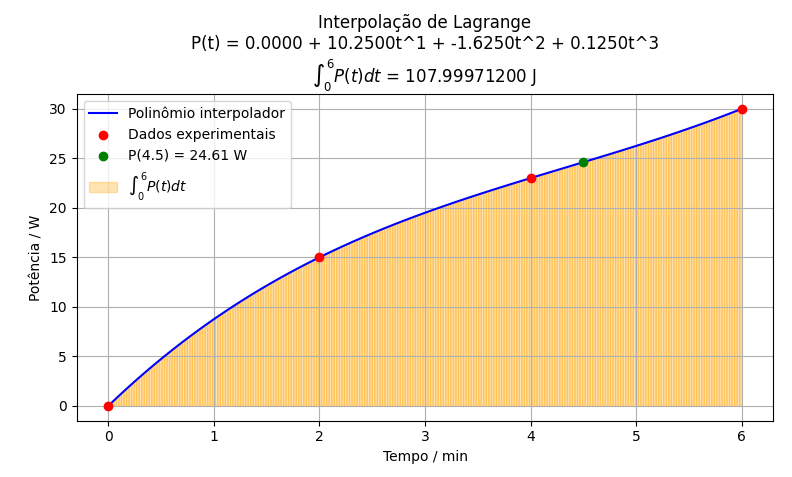
\includegraphics[width=1.0\textwidth, height=0.4\textheight, keepaspectratio]{Q2_resultados.png}
        \caption{Plotagem da integral da função}\label{fig:Q2_resultado}
\end{figure}

\begin{itemize}
    \item $P(t) = 0.0000 + 10.2500\,t - 1.6250\,t^2 + 0.1250\,t^3$
    \item $P(4.5) = 24.6094$ W (Watts)
    \item \textbf{Área sob o gráfico} = 107.9997 $\approx 108\ $ J (Joules)
\end{itemize}

A interpolação polinomial é amplamente utilizada em problemas de engenharia onde se necessita estimar valores intermediários entre dados experimentais, pois ela permite encontrar um curva que descreve a passagem pelos dados experimentais.

\subsection*{Aplicações na Engenharia Elétrica}
\justifying
Na engenharia elétrica, a interpolação é essencial para a análise de eficiência energética e caracterização de componentes. Dispositivos semicondutores, como diodos e transistores, e fontes de energia, como painéis fotovoltaicos, possuem curvas de operação não lineares 
(e.g., curvas de Corrente vs. Tensão, I-V). A partir de um conjunto discreto de medições experimentais, a interpolação polinomial permite construir uma função contínua que modela o comportamento do dispositivo em qualquer ponto de operação.

\section*{Questão 3:  Calculo de esforço total em fundacão com integração numérica}
\justifying
\subsection*{Contexto e Metodologia}

A integração numérica é fundamental em problemas onde não é possível obter soluções analíticas exatas das EDOs. Neste estudo, foram avaliados os métodos numéricos do Trapézio, Simpson 1/3 e Simpson 3/8 para calcular a $\int \left(150 + 30\sin\left(\frac{{\pi x}}{{3}}\right)\right) dx$ no intervalo [0,3].

\subsection*{Resultados Comparativos}
Foram testadas quatro quantidades distintas de subdivisões (n = 4, 20 e 100) e seu valor mínimo para convergência para cada método, foram aplicados zooms nos graficos plotados para que fosse possível visualizar o comportamento dos metodos de integração.

\begin{itemize}
    \item \textbf{n = 4}:
    \begin{figure}[H]
        \centering
        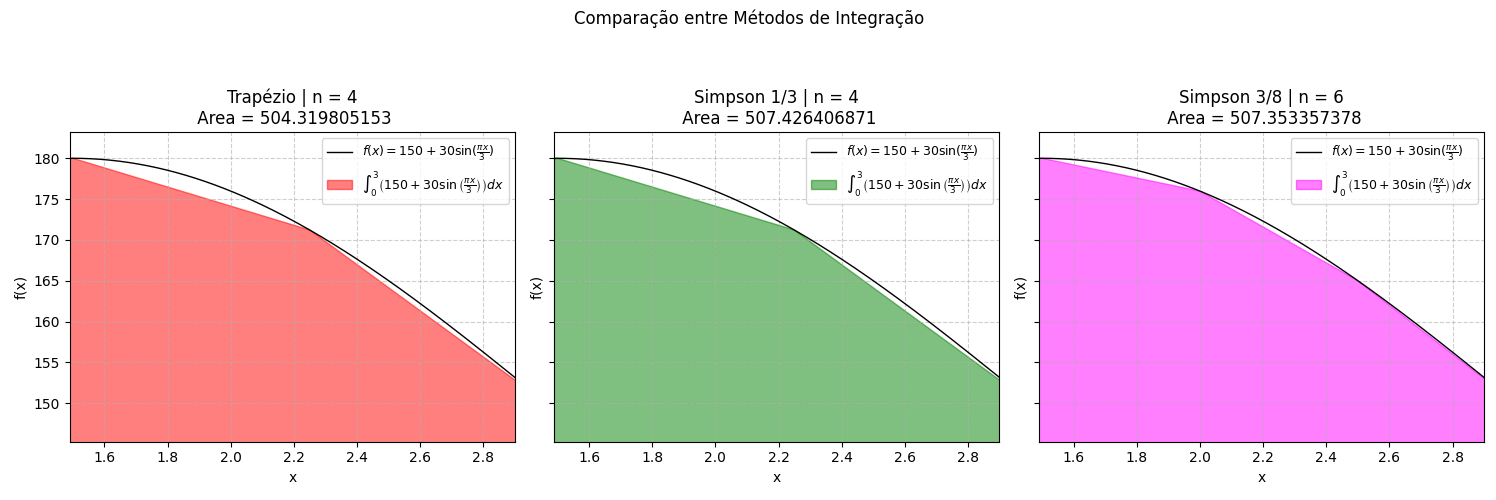
\includegraphics[width=1.0\textwidth, height=0.4\textheight, keepaspectratio]{n4.png}
        \caption{\small Comparação visual dos métodos de integração para n=4}\label{fig:n4}
    \end{figure}
    
    \item \textbf{n = 20}:
    \vspace{-1cm}
    \begin{figure}[H]
        \centering
        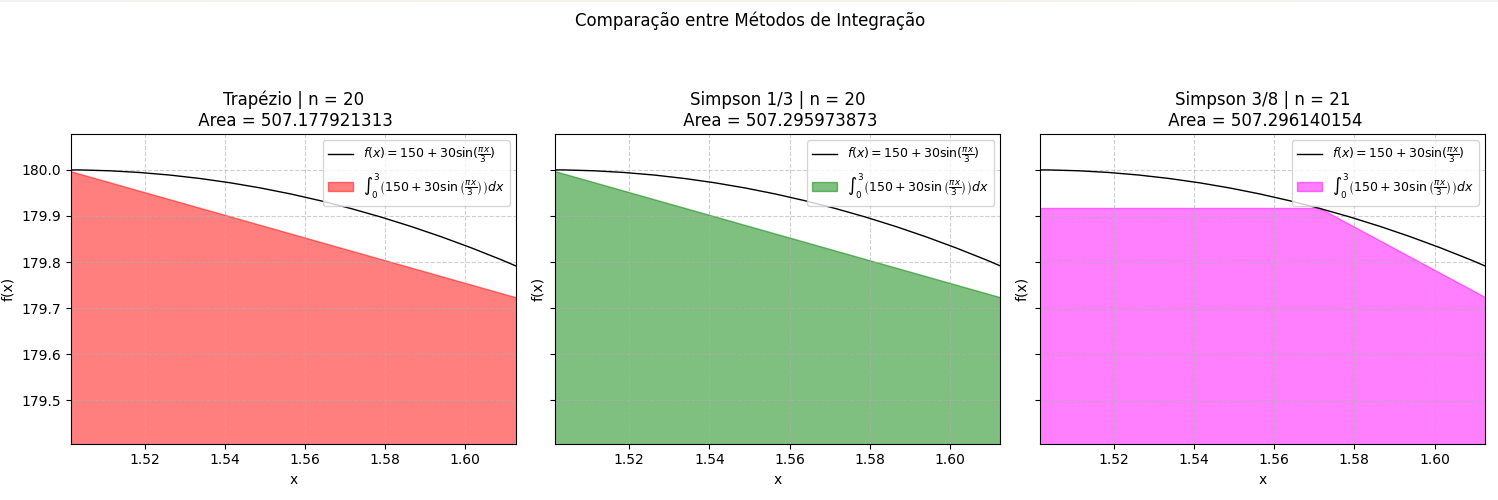
\includegraphics[width=1\textwidth, height=0.3\textheight, keepaspectratio]{n20.png}
        \caption{Comparação visual dos métodos de integração para n=20}\label{fig:n20}
    \end{figure}
    
    \item \textbf{n = 100}:
    \begin{figure}[H]
        \centering
        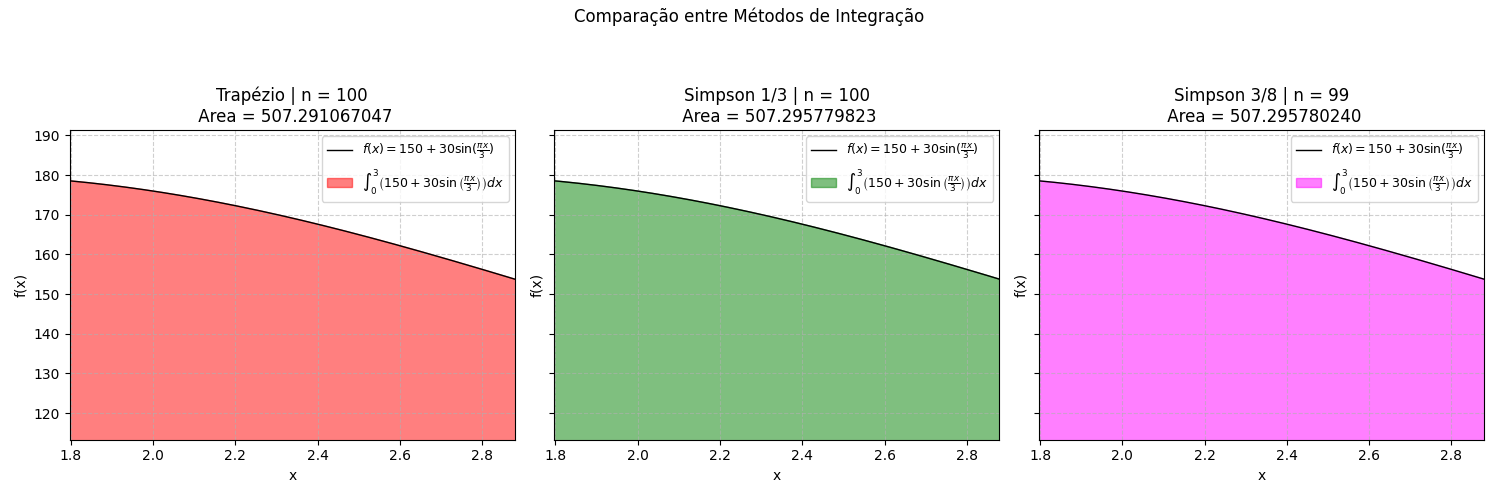
\includegraphics[width=1\textwidth, height=0.3\textheight, keepaspectratio]{n100.png}
        \caption{Comparação visual dos métodos de integração para n=100}\label{fig:n100}
    \end{figure}

    \item \textbf{n mínimo para convergência com precisão de 1e-5 do valor numérico}
    \begin{figure}[H]
        \centering
        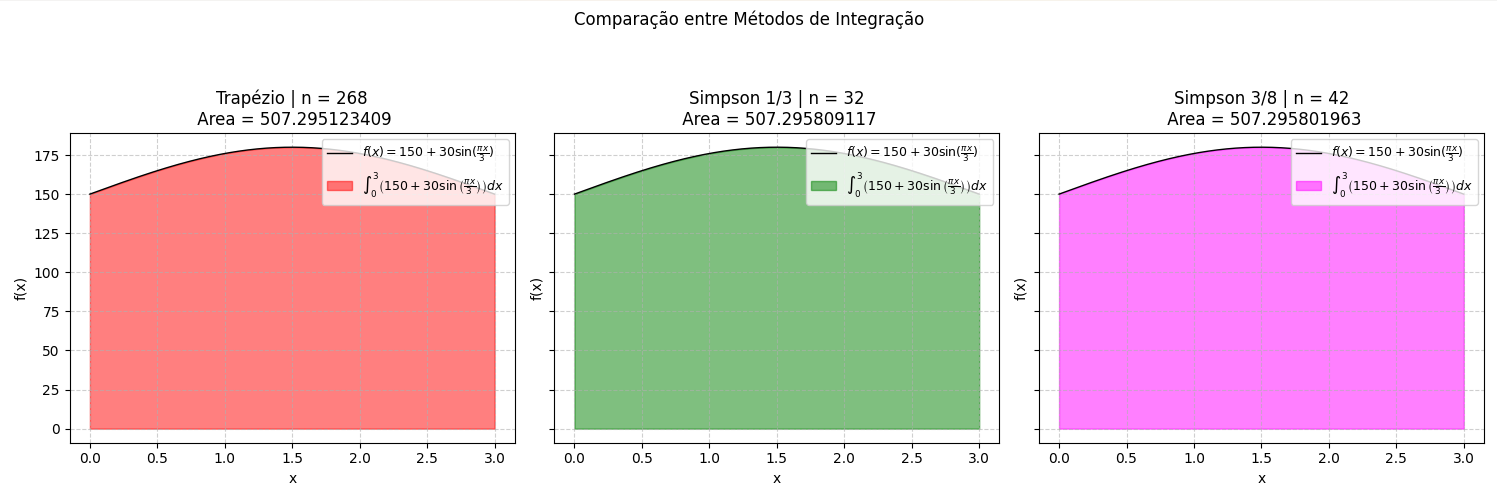
\includegraphics[width=1\textwidth, height=0.3\textheight, keepaspectratio]{n_min.png}
        \caption{Comparação visual dos métodos de integração para n específicos de cada método}\label{fig:n_min}
    \end{figure}
\end{itemize}

\begin{table}[htbp]
    \centering
    \caption{Comparativo das áreas calculadas para diferentes métodos e subdivisões.}\label{tab:resultados_agrupados}
    \begin{tabular}{c l r}
        \toprule
        \textbf{n} & \textbf{Método} & \textbf{ Tensão (kPa) } \\
        \midrule
        % --- Grupo para n=4 ---
        \multirow{3}{*}{4} 
        & Trapézio & 504.319805153 \\
        & Simpson 1/3 & 507.426406871 \\
        & Simpson 3/8 (n=6) & 507.353357378 \\
        \midrule
        % --- Grupo para n=20 ---
        \multirow{3}{*}{20} 
        & Trapézio & 507.177921313 \\
        & Simpson 1/3 & 507.295973873 \\
        & Simpson 3/8 (n=21) & 507.296140154 \\
        \midrule
        % --- Grupo para n=100 ---
        \multirow{3}{*}{100} 
        & Trapézio & 507.291067047 \\
        & Simpson 1/3 & 507.295779823 \\
        & Simpson 3/8 (n=99) & 507.295780240 \\
        \midrule
        268 & Trapézio & 507.295123409 \\
        32 & Simpson 1/3 & 507.295809117 \\
        42 & Simpson 3/8 & 507.295801963 \\
        \bottomrule
    \end{tabular}
\end{table}
\vspace{2cm}

\subsection*{Análise de Convergência}
Foi utilizado a seguinte função para identificar os valores de n mínimo para atingir a convergência com uma tolerancia de 1e-5. Com ele foi possível encontrar os valores de n, os quais mostram que, para essa função $f(x) = 150 + 30\sin(\frac{\pi x}{3})$ o método de Simpson 1/3 precisou de uma quantidade menor de passos para atingir o valor númerico da integral dentro do intervalo.
\begin{figure}[H]
    \begin{lstlisting}[caption={Função para encontrar o número mínimo de passos para convergência.}, label={lst:find_steps}]
        def find_min_steps(
        func, 
        method, 
        lower_bound, 
        upper_bound, 
        tolerance=1e-5, 
        max_steps=1e4) -> int:
            if method == simpsons_3_8:
                steps = 3
                prev_area = method(func, lower_bound, upper_bound, steps)
                while steps <= max_steps:
                    steps += 3
                    current_area = method(func, lower_bound, upper_bound, steps)
                    
                    if abs(current_area - prev_area) < tolerance:
                        return steps
                    
                    prev_area = current_area
                return None
            else:
                steps = 2
                prev_area = method(func, lower_bound, upper_bound, steps)
                
                while steps <= max_steps:
                    steps += 2
                    current_area = method(func, lower_bound, upper_bound, steps)
                    
                    if abs(current_area - prev_area) < tolerance:
                        return steps
                    
                    prev_area = current_area
                return None
    \end{lstlisting}
\end{figure}

\subsection*{Eficiência Numérica}
\begin{itemize}
    \item \textbf{Trapézio}: Demonstrou ser o método menos eficiente, exigindo 268 subdivisões para atingir a convergência. Embora sua aproximação melhore com o aumento de n, a taxa de convergência é notavelmente lenta, confirmando que este método requer um esforço computacional significativamente maior para alcançar alta precisão em funções com curvatura.

    \item \textbf{Simpson 1/3}: Apresentou um desempenho muito superior, convergindo com apenas 32 subdivisões. Isso indica que o método é mais de 8 vezes mais rápido que o método do Trapézio para atingir a mesma precisão. Sua eficiência deriva da aproximação da função por polinômios de grau 2 (parábolas), que modelam a geometria da função senoide de forma muito mais eficaz que as retas do método do Trapézio.

    \item \textbf{Simpson 3/8}: Atingiu a convergência com 42 subdivisões, um resultado também drasticamente superior ao do Trapézio e competitivo com o de Simpson 1/3. Embora neste caso específico tenha exigido um pouco mais de passos que o Simpson 1/3, sua eficiência é da mesma ordem de magnitude. A principal restrição do método continua sendo a necessidade de um número de subintervalos múltiplo de 3.

\end{itemize}
\subsection*{Discretização e Confiabilidade}
\begin{itemize}
    \item \textbf{Passo pequenos}: os erros são significativos pois a quantidade de passos para a convergência é muito baixa, fazendo com que os metodos não atijam a precisão desejada
    \item A escolha do Simpson 1/3 com n $\geq$ 32 garante precisão e eficiência, evitando superdimensionamento ou falhas. Já o método do Trapézio, mesmo com n=100, ainda tem erro residual, enquanto os métodos de Simpson atingem tolerância desejada com menos passos.

\end{itemize}

\subsection*{Conclusão}
A precisão no cálculo da força total em fundações é essencial para segurança, economia e conformidade normativa. O método de Simpson 1/3 mostrou-se o mais confiável para a função analisada, equilibrando precisão e eficiência. Já a discretização inadequada (ex.: 
n=4 no Trapézio) compromete a confiabilidade, evidenciando a necessidade de critérios rigorosos na seleção do método e do número de subdivisões.

Os métodos de Simpson mostraram-se mais eficientes para esta função, especialmente quando o número de subdivisões é pequeno. O trapézio, embora mais simples, exige mais avaliações para atingir a mesma precisão. A escolha do método deve considerar:
\begin{itemize}
\item Natureza da função (suavidade, periodicidade)
\item Custo computacional de cada avaliação da função
\item Precisão requerida na aplicação prática
\end{itemize}

\end{document}